\documentclass[12pt]{article}
\usepackage[utf8]{inputenc}
\usepackage{parskip}
\usepackage{markdown}
\usepackage{hyperref}
\usepackage{listings}
\usepackage{color}
\usepackage[subtle]{savetrees}
\usepackage{verbatim}
\usepackage{blindtext}

\title{\vspace{-2cm} \textbf{Session 4 - Let's Do Some Maths! v.2} \\ UCAS Program 2020}

\author{Chloe Lau}
\date{August 2020}

\begin{document}
\setlength{\parindent}{4ex}
\setlength{\parskip}{1em}

\maketitle

\section{After the last "Let's Do Some Maths!"...}
What have you benefited from it? Did you try \textbf{thinking out loud}? Did you practice with more Mathematical Problems?

Today we will continue with some interesting Mathematical problems, but in a way more interesting manner.

\section{Let's Do Some Maths! - With A Twist}
So you've tried writing out all your thinking processes, then constructing an explanation to your peers, now, I would like you to solve the questions in pairs.

In each pair, one student would have to attempt one question out of the two, with their full thinking process laid out. The other student would be leading the student and making sure the student's words makes sense.

You will be given 15 minutes per task, with a 5 minute reflection time on how well you have explained your own train of thoughts.


\newpage
\subsection{MAT 2008, Q5}
\begin{center}
    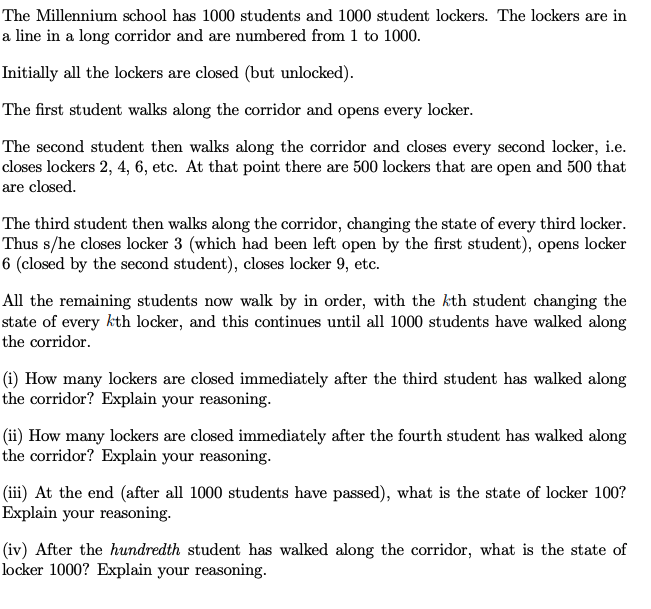
\includegraphics[scale=0.55]{mat08-5.png}
\end{center}

Space for some scribbling:

\newpage
\subsection{Underground Mathematics, Triominoes}
\setlength{\parindent}{0pt}
\begin{center}
    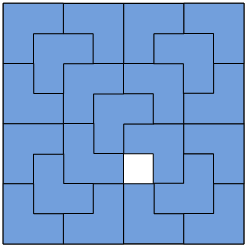
\includegraphics[scale=0.55]{triominos.png}
\end{center}
A board is divided into squares the same size as of the $\frac 1 3$ tiles. A triomino is 3-squared, L-shaped. The board is $2^n$ by $2^n$ squares.

One square, anywhere on the board, is coloured white.

We can put triominoes on the board, but they must not overlap and must not cover the blue square.

Is it possible to cover the board (apart from the blue square) with triominoes? Does it depend on where the blue square is, or on the n that determines the size of the board? Justify your answer.

\setlength{\parindent}{4ex}
Space for some scribbling:
\end{document}
